

\section{montecarlo bootstrapping }

Monte Carlo bootstrapping is used to find the model for the mpg data. It starts by cleaning the data, then selecting the numeric columns, and defining the Monte Carlo bootstrapping function. After that, it defines the polynomial regression function using mpg as the dependent variable. Next, it defines the simulation function using clusters, thereby speeding up the computation time with the doParallel library. After defining the run simulation function, it runs the simulation with the set seed, simulation number, and sample size of the Monte Carlo bootstrapping method.

After that, it creates histograms of the simulation results. It calculates the mean result of the coefficients, and using these means, it calculates a new regression model and the R-squared of the new average model. Finally, it makes a scatter plot showing the final regression model results versus the results from the actual data set.

\lstinputlisting[language=R, caption=montecarlo bootstrapping]{C:/Users/Jonathan/Documents/GitHub/P2/R kode/montecarlo bootstrapping.R}

\begin{figure}[h] 
	\centering
	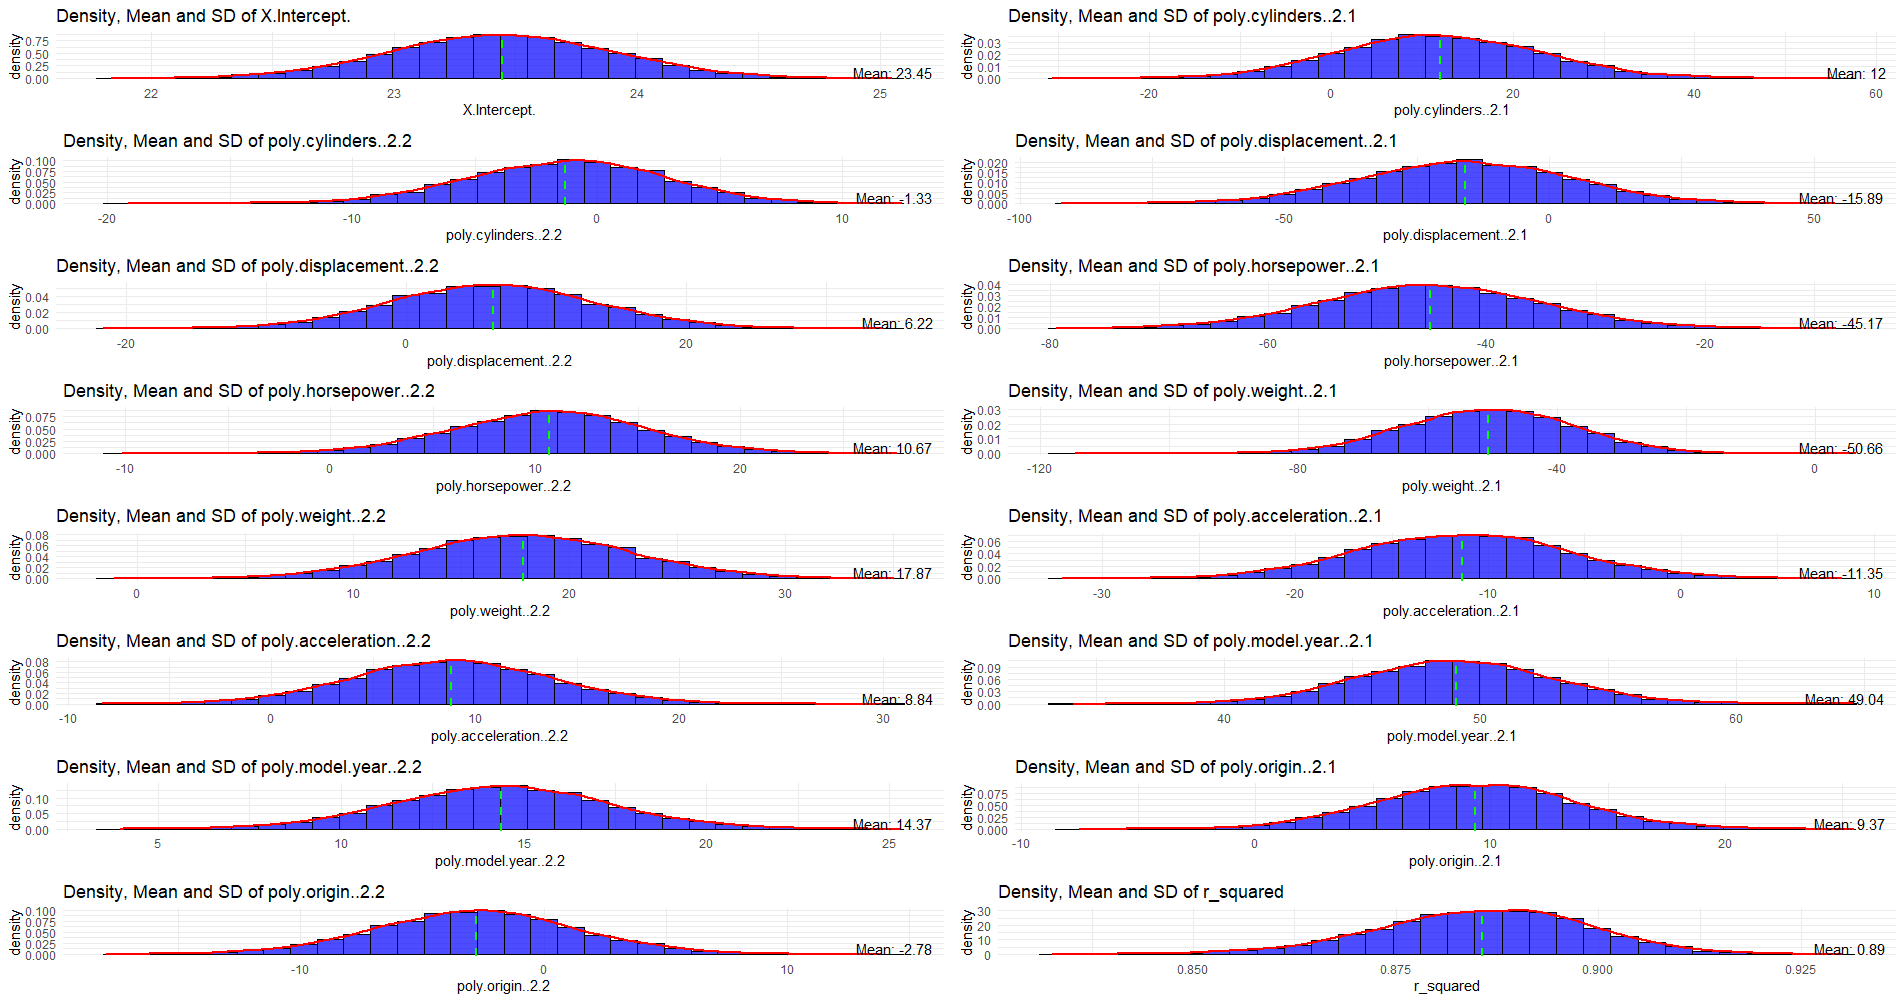
\includegraphics[width=14cm]{C:/Users/Jonathan/Documents/GitHub/P2/latex/p2/10.png}
	\caption{AQI gennem årene.}
	\label{fig:j06}
\end{figure}

\begin{figure}[h] 
	\centering
	\includegraphics[width=14cm]{C:/Users/Jonathan/Desktop/p2/11.png}
	\caption{AQI gennem årene.}
	\label{fig:j06}
\end{figure}